%----------------------------------------------------------------------------------------
%	Paquetes y configuración
%----------------------------------------------------------------------------------------
\documentclass{article}

\usepackage[utf8]{inputenc}
\usepackage[spanish,es-lcroman]{babel}
\usepackage{fancyhdr}
\usepackage{lastpage}
\usepackage{extramarks}
\usepackage[usenames,dvipsnames]{color}
\usepackage{graphicx}
\usepackage{listings}
\usepackage{xparse}
\usepackage{courier}
\usepackage{amsmath}
\usepackage{enumitem}
\usepackage{hyperref}
\usepackage{mathtools}
\usepackage{lipsum}
\usepackage{float}
\usepackage{algorithm}
\usepackage{algpseudocode}
\usepackage{booktabs}
\usepackage{MnSymbol}
\usepackage{subcaption}
\floatplacement{figure}{H}

% Margenes
\topmargin=-0.45in
\evensidemargin=0in
\oddsidemargin=0in
\textwidth=6.5in
\textheight=9.0in
\headsep=0.25in

\renewcommand{\arraystretch}{1.2}

% Header y footer
\pagestyle{fancy}
\lhead{}
\chead{\tareaRamo\ (\tareaProfesor): \tareaTitulo} % Centro
\rhead{\firstxmark}
\lfoot{UTFSM CSJ - Departamento de Informática}
\cfoot{}
\rfoot{Página\ \thepage\ de\ \protect\pageref{LastPage}} % Pagina
\renewcommand\headrulewidth{0.4pt}
\renewcommand\footrulewidth{0.4pt}

% \setlength\parindent{0pt} % Eliminar la indentación

%----------------------------------------------------------------------------------------
%	Inclusión de python con systax highlight
%----------------------------------------------------------------------------------------
\renewcommand\lstlistingname{Script}
\renewcommand\lstlistlistingname{Scripts}

\definecolor{MyDarkGreen}{rgb}{0.0,0.4,0.0}
\lstset{prebreak=\raisebox{0ex}[0ex][0ex]
        {\ensuremath{\rhookswarrow}}}
\lstset{postbreak=\raisebox{0ex}[0ex][0ex]
        {\ensuremath{\rcurvearrowse\space}}}
\lstset{breaklines=true, breakatwhitespace=true}
\lstset{numbers=left, numberstyle=\scriptsize}
\lstloadlanguages{Python}
\lstset{
  language=Python,
  frame=single, % Single frame around code
  basicstyle=\small\ttfamily, % Use small true type font
  keywordstyle=[1]\color{BlueViolet}\bf, % Function names
  keywordstyle=[2]\color{Purple}, % Arguments
  keywordstyle=[3]\color{Blue}\underbar,
  identifierstyle=,
  commentstyle=\usefont{T1}{pcr}{m}{sl}\color{MyDarkGreen}\small,
  stringstyle=\color{Purple},
  showstringspaces=false,
  tabsize=5,
  morekeywords={rand,},
  morekeywords=[2]{on, off, interp},
  morekeywords=[3]{y, range},
  morecomment=[l][\color{Blue}]{...},
  numbers=left,
  firstnumber=1,
  numberstyle=\tiny\color{Gray},
  stepnumber=1
}

\newcommand{\python}[2]{
  \begin{itemize}
    \item[]\lstinputlisting[language=Python,caption=#2,label=#1]{#1.py}
  \end{itemize}
}

\newcommand{\bash}[2]{
  \begin{itemize}
    \item[]\lstinputlisting[language=Bash,caption=#2,label=#1]{#1.sh}
  \end{itemize}
}

%----------------------------------------------------------------------------------------
%	Meta Información
%----------------------------------------------------------------------------------------
\newcommand{\tareaTitulo}{Tarea\ 2}
\newcommand{\tareaFecha}{\today}
\newcommand{\tareaRamo}{INF391 Reconocimiento\ de\ Patrones\ en\ Minería\ de\ Datos}
\newcommand{\tareaProfesor}{Marcelo\ Mendoza}

%----------------------------------------------------------------------------------------
%	Título
%----------------------------------------------------------------------------------------
\title{
  \Large\textmd{\textbf{\tareaRamo\\ \tareaTitulo}}\\
  \vspace{0.1in}
  \normalsize
  Universidad Técnica Federico Santa María, Campus San Joaquín\\
  Departamento de Informática\\
  \vspace{0.1in}
  \small{\textsc{\tareaFecha}}\\
  \vspace{0.1in}
  \large{\textsc{Profesor Marcelo Mendoza}}
  \vspace{1.5in}
}

\author{
    \textit{Juan Pablo Escalona} \\
    \small{juan.escalonag@alumnos.usm.cl} \\
    \small{201073515-k}
    \and
    \textit{Rafik Masad} \\
    \small{rafik.masad@alumnos.usm.cl} \\
    \small{201073519-2}
    \and
    \textit{Gianfranco Valentino}\\
    \small{gianfranco.valentino@alumnos.usm.cl}\\
    \small{2860574-9}
}
\date{}

%----------------------------------------------------------------------------------------
% Documento
%----------------------------------------------------------------------------------------
\begin{document}

\maketitle
\newpage

%----------------------------------------------------------------------------------------
% Índice
%----------------------------------------------------------------------------------------
% \setcounter{tocdepth}{3}
% \newpage
% \tableofcontents
% \newpage

%----------------------------------------------------------------------------------------
% Desarrollo
%----------------------------------------------------------------------------------------
\section{Introducción}
En el presente informe, se pretende analizar dos algoritmos que permiten encontrar reglas de asociación sobre un historial de transacciones. Estos algoritmos, Apriori y FP-Growth, se basan en parámetros como Confianza(Conf) y Soporte Mínimo(MinSup). Otros parámetros, permiten limitar el número máximo de reglas encontradas, para terminar la ejecución de forma temprana.

Se buscarán reglas interesantes, y ademas se pretende comparar tiempos de ejecución, para observar la eficiencia de ambos algoritmos, frente a distintas condiciones.

Para el desarrollo de la experiencia se escribió un script en python capaz de ejecutar los diferentes algoritmos con los parámetros a probar utilizando WEKA. Este script genera gráficos interesantes de salida, los cuales se analizan en el informe. Todos los scripts creados para esta experiencia se encuentran en~\ref{anexo}.

\section{Algoritmo Apriori}

En este experimento se gráfica la confianza entre 0.85 y 0.95 utilizando un soporte mínimo de 0.1 y 0.15. En el eje Y se presenta el número de reglas encontradas para cada una de las confianzas.

\subsection{Gráficos de confianza y soporte mínimo}

\begin{figure}[H]
  \begin{subfigure}[b]{0.49\textwidth}
    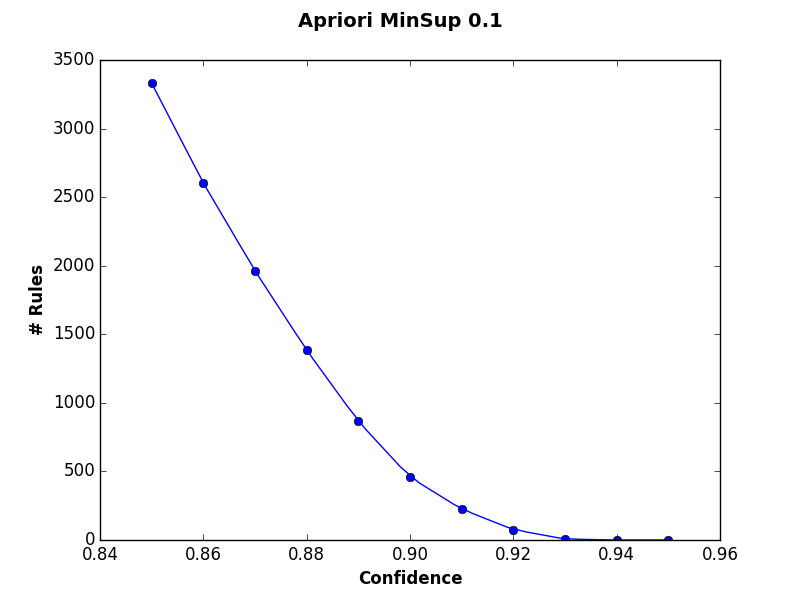
\includegraphics[width=\linewidth]{{src/img/Apriori-0.1}.png}
    \caption{Algoritmo Apriori: Confianza vs Número de reglas encontradas con soporte mínimo 0.1}
    \label{grafico:apriori:1}
  \end{subfigure}
  %
  \begin{subfigure}[b]{0.5\textwidth}
    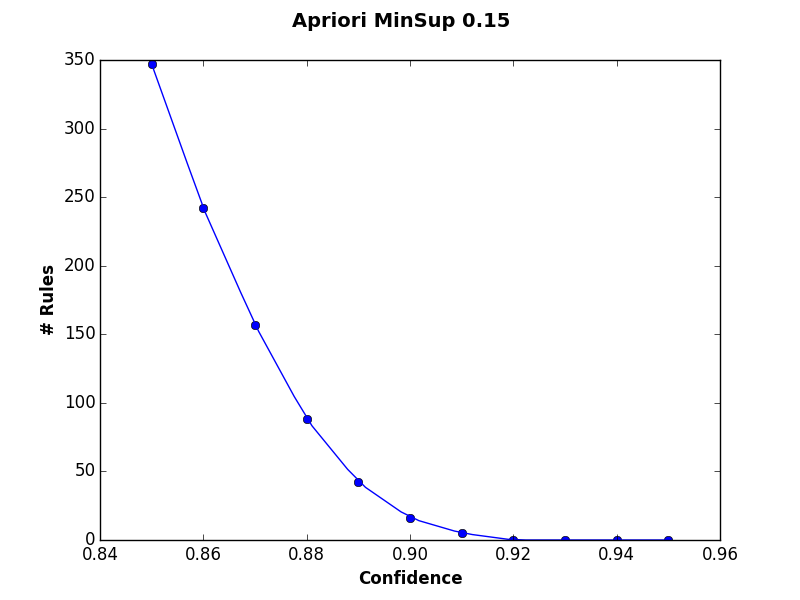
\includegraphics[width=\linewidth]{{src/img/Apriori-0.15}.png}
    \caption{Algoritmo Apriori: Confianza vs Número de reglas encontradas con soporte mínimo 0.15}
    \label{grafico:apriori:2}
  \end{subfigure}
\end{figure}

Es importante destacar la diferencia entre los ejes y de ambos gráficos, hay una diferencia en magnitud de orden 10.

\subsection{Gráficos de tiempo de ejecución}

\begin{figure}[H]
  \begin{subfigure}[b]{0.49\textwidth}
    \includegraphics[width=\linewidth]{{src/img/Apriori-0.1-exec-conf}.png}
    \caption{Algoritmo Apriori: Tiempo de ejecución para confianzas entre 0.85 y 0.95 con soporte mínimo de 0.1}
    \label{grafico:apriori-exec:1}
  \end{subfigure}
  %
  \begin{subfigure}[b]{0.5\textwidth}
    \includegraphics[width=\linewidth]{{src/img/Apriori-0.15-exec-conf}.png}
    \caption{Algoritmo Apriori:  Tiempo de ejecución para confianzas entre 0.85 y 0.95 con soporte mínimo de 0.15}
    \label{grafico:apriori-exec:2}
  \end{subfigure}
\end{figure}

\section{Algoritmo FP-Growth}

Para este experimento se hace variar la confianza mínima entre 0.85 a 0.95 para cada uno de los soportes mínimos entre 0.16 y 0.25. Se generan entonces 10 gráficos con diferentes soportes mínimos, en el eje X se presenta la confianza entre 0.85 y 0.95. El eje Y representa el número de reglas encontradas.

\subsection{Gráficos de confianza y soporte mínimo}

\begin{figure}[H]
  \centering
  \begin{subfigure}[b]{0.49\textwidth}
    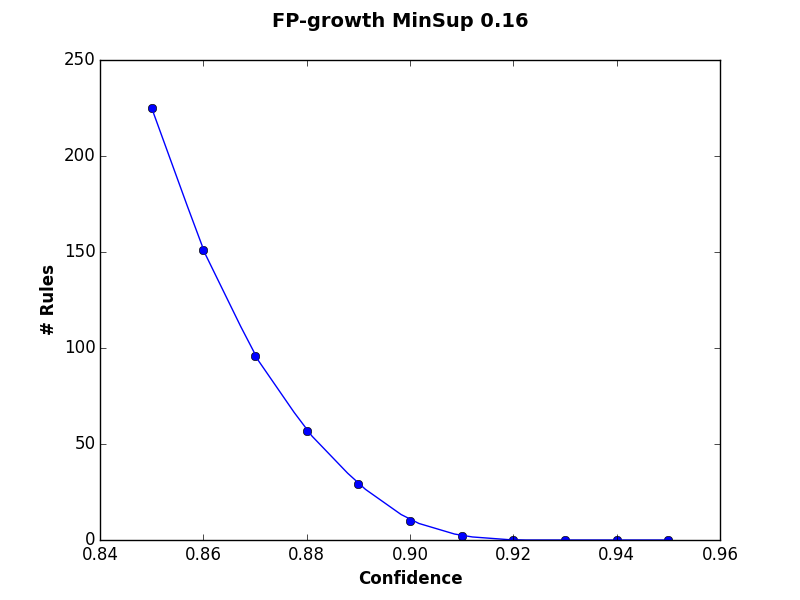
\includegraphics[width=\linewidth]{{src/img/FP-growth-0.16}.png}
    \caption{Algoritmo FP-growth: Confianza vs Número de reglas encontradas con soporte mínimo 0.16}
    \label{grafico:FPgrowth:16}
  \end{subfigure}
  %
  \begin{subfigure}[b]{0.49\textwidth}
    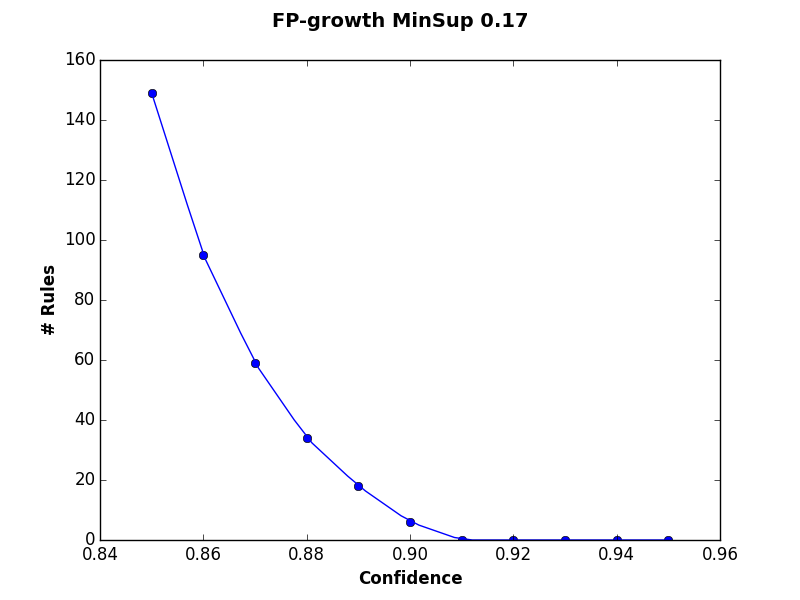
\includegraphics[width=\linewidth]{{src/img/FP-growth-0.17}.png}
    \caption{Algoritmo FP-growth: Confianza vs Número de reglas encontradas con soporte mínimo 0.17}
    \label{grafico:FPgrowth:17}
  \end{subfigure}
\end{figure}

\begin{figure}[H]
  \centering
  \begin{subfigure}[b]{0.49\textwidth}
    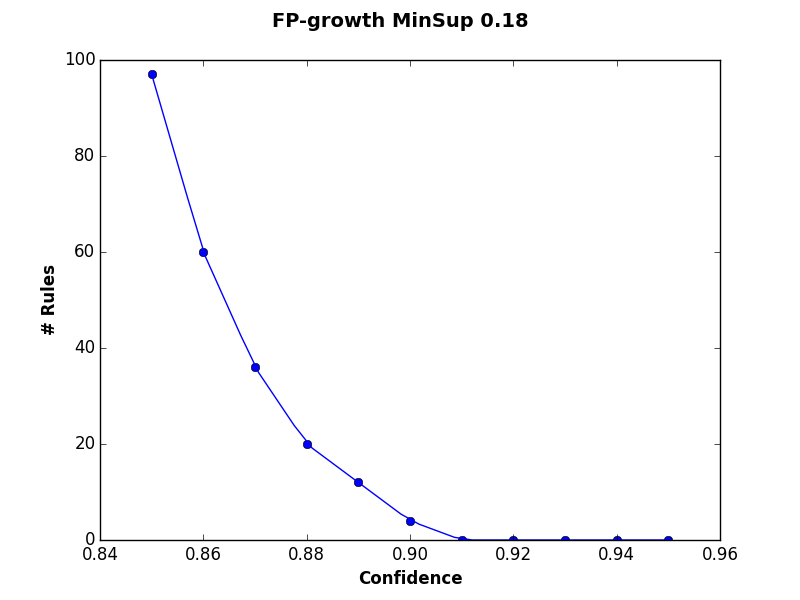
\includegraphics[width=\linewidth]{{src/img/FP-growth-0.18}.png}
    \caption{Algoritmo FP-growth: Confianza vs Número de reglas encontradas con soporte mínimo 0.18}
    \label{grafico:FPgrowth:18}
  \end{subfigure}
  %
  \begin{subfigure}[b]{0.49\textwidth}
    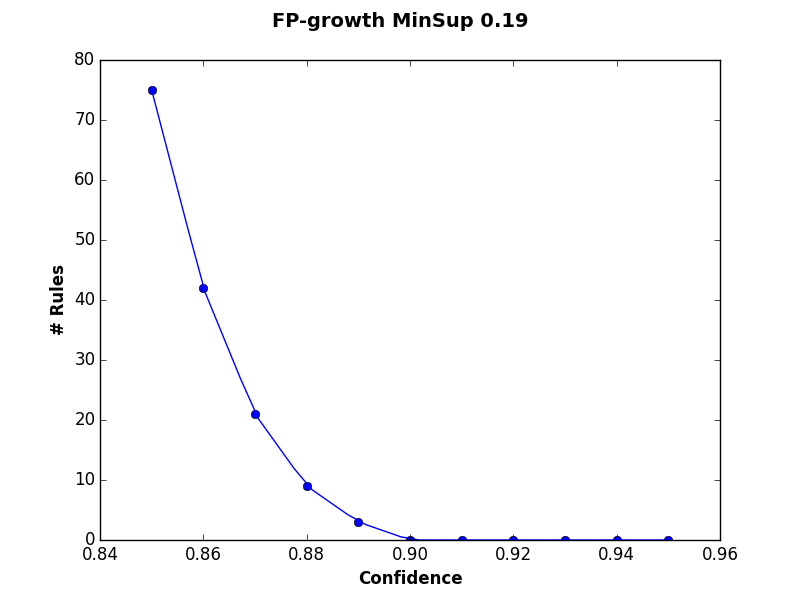
\includegraphics[width=\linewidth]{{src/img/FP-growth-0.19}.png}
    \caption{Algoritmo FP-growth: Confianza vs Número de reglas encontradas con soporte mínimo 0.19}
    \label{grafico:FPgrowth:19}
  \end{subfigure}
\end{figure}

\begin{figure}[H]
  \centering
  \begin{subfigure}[b]{0.49\textwidth}
    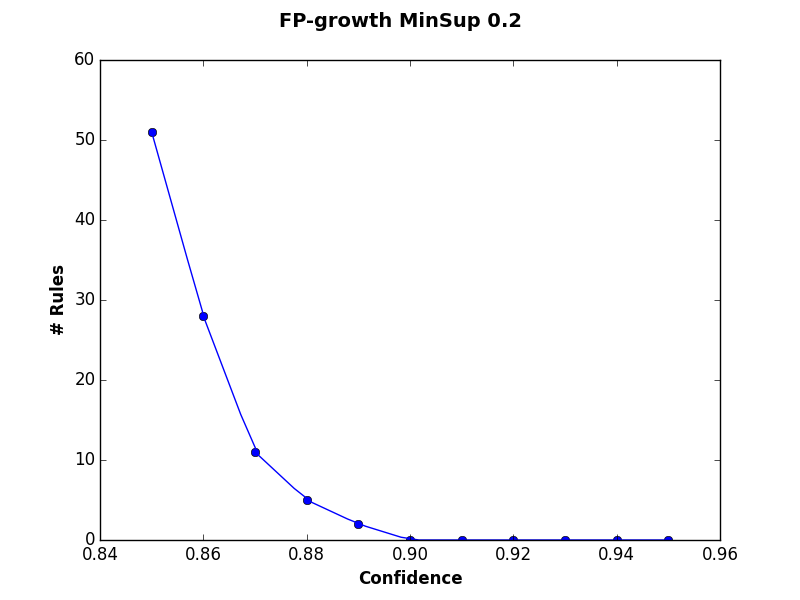
\includegraphics[width=\linewidth]{{src/img/FP-growth-0.2}.png}
    \caption{Algoritmo FP-growth: Confianza vs Número de reglas encontradas con soporte mínimo 0.20}
    \label{grafico:FPgrowth:20}
  \end{subfigure}
  %
  \begin{subfigure}[b]{0.49\textwidth}
    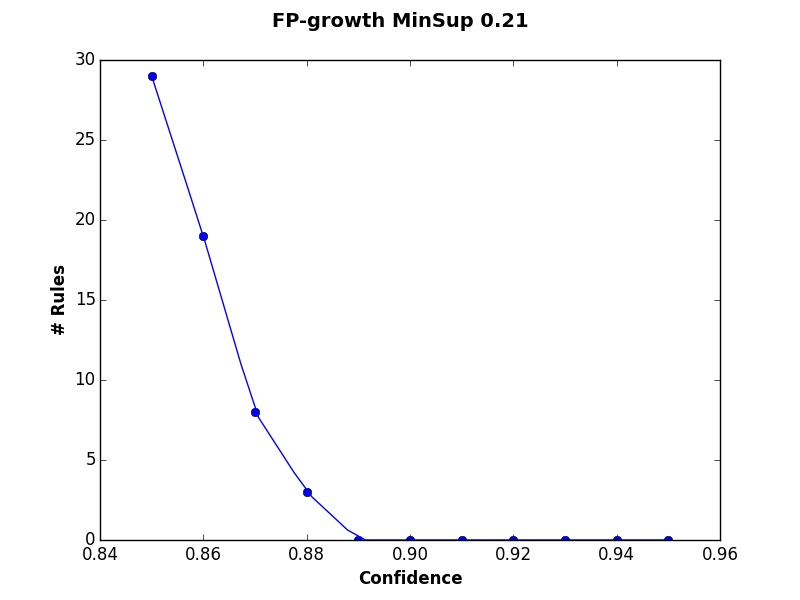
\includegraphics[width=\linewidth]{{src/img/FP-growth-0.21}.png}
    \caption{Algoritmo FP-growth: Confianza vs Número de reglas encontradas con soporte mínimo 0.21}
    \label{grafico:FPgrowth:21}
  \end{subfigure}
\end{figure}

\begin{figure}[H]
  \centering
  \begin{subfigure}[b]{0.49\textwidth}
    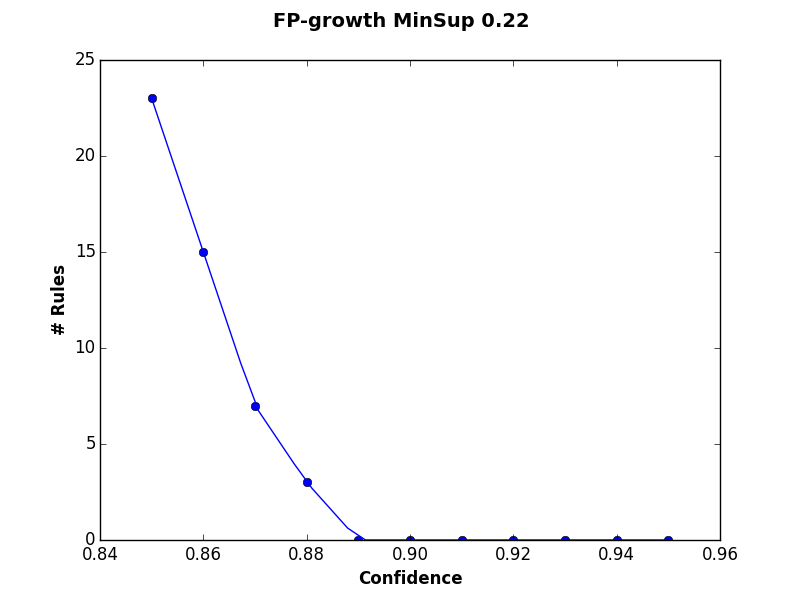
\includegraphics[width=\linewidth]{{src/img/FP-growth-0.22}.png}
    \caption{Algoritmo FP-growth: Confianza vs Número de reglas encontradas con soporte mínimo 0.22}
    \label{grafico:FPgrowth:22}
  \end{subfigure}
  %
  \begin{subfigure}[b]{0.49\textwidth}
    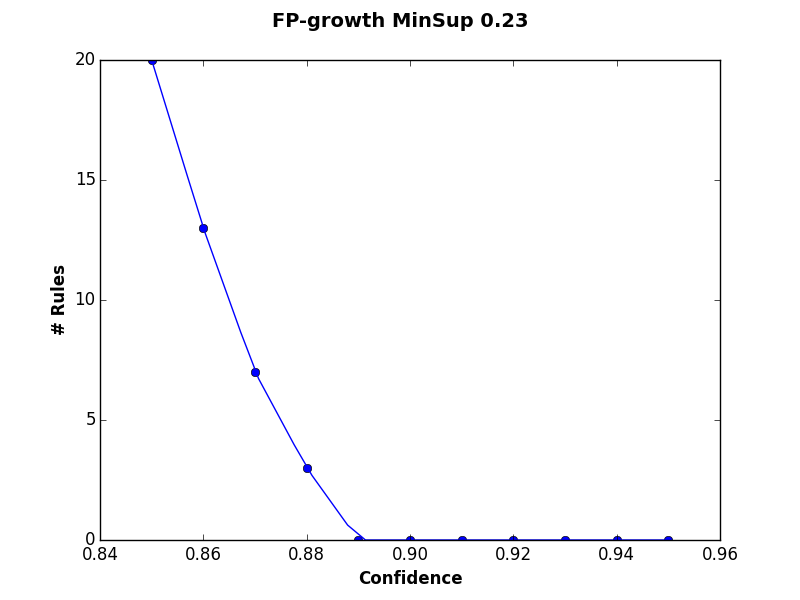
\includegraphics[width=\linewidth]{{src/img/FP-growth-0.23}.png}
    \caption{Algoritmo FP-growth: Confianza vs Número de reglas encontradas con soporte mínimo 0.23}
    \label{grafico:FPgrowth:23}
  \end{subfigure}
\end{figure}

\begin{figure}[H]
  \centering
  \begin{subfigure}[b]{0.49\textwidth}
    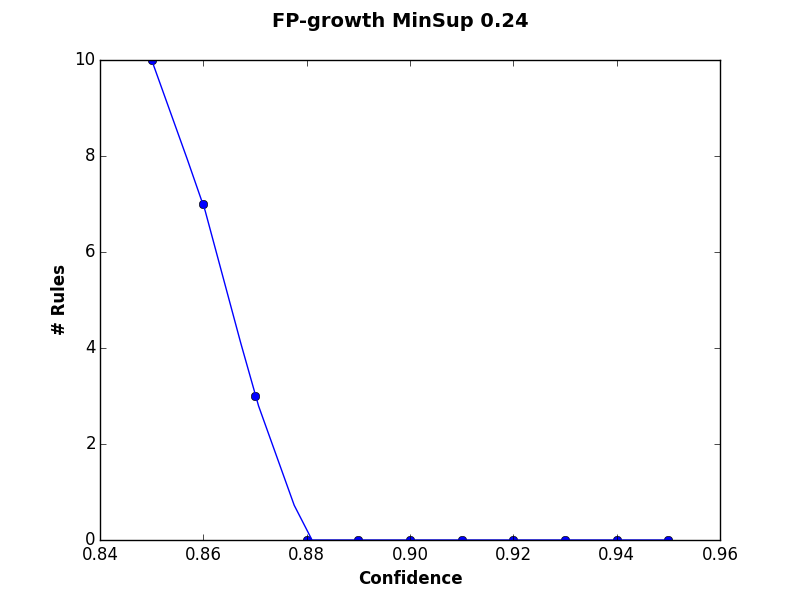
\includegraphics[width=\linewidth]{{src/img/FP-growth-0.24}.png}
    \caption{Algoritmo FP-growth: Confianza vs Número de reglas encontradas con soporte mínimo 0.24}
    \label{grafico:FPgrowth:24}
  \end{subfigure}
  %
  \begin{subfigure}[b]{0.49\textwidth}
    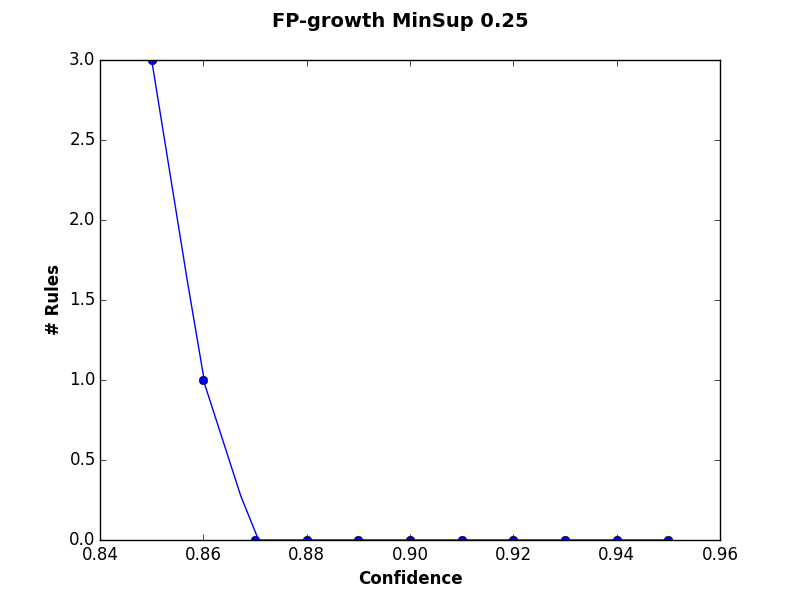
\includegraphics[width=\linewidth]{{src/img/FP-growth-0.25}.png}
    \caption{Algoritmo FP-growth: Confianza vs Número de reglas encontradas con soporte mínimo 0.25}
    \label{grafico:FPgrowth:25}
  \end{subfigure}
\end{figure}

\subsection{Gráficos de tiempo de ejecución}

\begin{figure}[H]
  \centering
  \begin{subfigure}[b]{0.49\textwidth}
    \includegraphics[width=\linewidth]{{src/img/FP-growth-0.16-exec-conf}.png}
    \caption{Algoritmo FP-growth: Confianza vs Número de reglas encontradas con soporte mínimo 0.16}
    \label{grafico:FPgrowth-exec:16}
  \end{subfigure}
  %
  \begin{subfigure}[b]{0.49\textwidth}
    \includegraphics[width=\linewidth]{{src/img/FP-growth-0.17-exec-conf}.png}
    \caption{Algoritmo FP-growth: Confianza vs Número de reglas encontradas con soporte mínimo 0.17}
    \label{grafico:FPgrowth-exec:17}
  \end{subfigure}
\end{figure}

\begin{figure}[H]
  \centering
  \begin{subfigure}[b]{0.49\textwidth}
    \includegraphics[width=\linewidth]{{src/img/FP-growth-0.18-exec-conf}.png}
    \caption{Algoritmo FP-growth: Confianza vs Número de reglas encontradas con soporte mínimo 0.18}
    \label{grafico:FPgrowth-exec:18}
  \end{subfigure}
  %
  \begin{subfigure}[b]{0.49\textwidth}
    \includegraphics[width=\linewidth]{{src/img/FP-growth-0.19-exec-conf}.png}
    \caption{Algoritmo FP-growth: Confianza vs Número de reglas encontradas con soporte mínimo 0.19}
    \label{grafico:FPgrowth-exec:19}
  \end{subfigure}
\end{figure}

\begin{figure}[H]
  \centering
  \begin{subfigure}[b]{0.49\textwidth}
    \includegraphics[width=\linewidth]{{src/img/FP-growth-0.2-exec-conf}.png}
    \caption{Algoritmo FP-growth: Confianza vs Número de reglas encontradas con soporte mínimo 0.20}
    \label{grafico:FPgrowth-exec:20}
  \end{subfigure}
  %
  \begin{subfigure}[b]{0.49\textwidth}
    \includegraphics[width=\linewidth]{{src/img/FP-growth-0.21-exec-conf}.png}
    \caption{Algoritmo FP-growth: Confianza vs Número de reglas encontradas con soporte mínimo 0.21}
    \label{grafico:FPgrowth-exec:21}
  \end{subfigure}
\end{figure}

\begin{figure}[H]
  \centering
  \begin{subfigure}[b]{0.49\textwidth}
    \includegraphics[width=\linewidth]{{src/img/FP-growth-0.22-exec-conf}.png}
    \caption{Algoritmo FP-growth: Confianza vs Número de reglas encontradas con soporte mínimo 0.22}
    \label{grafico:FPgrowth-exec:22}
  \end{subfigure}
  %
  \begin{subfigure}[b]{0.49\textwidth}
    \includegraphics[width=\linewidth]{{src/img/FP-growth-0.23-exec-conf}.png}
    \caption{Algoritmo FP-growth: Confianza vs Número de reglas encontradas con soporte mínimo 0.23}
    \label{grafico:FPgrowth-exec:23}
  \end{subfigure}
\end{figure}

\begin{figure}[H]
  \centering
  \begin{subfigure}[b]{0.49\textwidth}
    \includegraphics[width=\linewidth]{{src/img/FP-growth-0.24-exec-conf}.png}
    \caption{Algoritmo FP-growth: Confianza vs Número de reglas encontradas con soporte mínimo 0.24}
    \label{grafico:FPgrowth-exec:24}
  \end{subfigure}
  %
  \begin{subfigure}[b]{0.49\textwidth}
    \includegraphics[width=\linewidth]{{src/img/FP-growth-0.25-exec-conf}.png}
    \caption{Algoritmo FP-growth: Confianza vs Número de reglas encontradas con soporte mínimo 0.25}
    \label{grafico:FPgrowth-exec-minsup:25}
  \end{subfigure}
\end{figure}

\begin{figure}[H]
  \centering
  \includegraphics[width=0.49\linewidth]{{src/img/FP-growth-0.25-exec-minsup}.png}
  \caption{Algoritmo FP-growth: tiempo de ejecución, Confianza vs Soportes mínimos}
  \label{grafico:FPgrowth-exec:25}
\end{figure}

\section{Reglas interesantes}

\subsubsection*{El monopolio del pan y pasteles}

En un alto porcentaje de las reglas encontradas, sobre todo las de más alto porcentaje de confianza, encontramos que una combinación de compras implica la compra de pan o pasteles. Lo anterior nos da a inferir que estos productos son altamente consumidos y un porcentaje alto de los consumidores al comprar algún producto llevan además pan o pasteles ya que es algo que es necesario constantemente en el hogar.

\subsubsection*{¿Vegetales?}

En una situación similar pero en menor medida a la de los panes y pasteles existen múltiples relaciones entre distintas combinaciones de compras y vegetales. En particular se repite bastante combinaciones que incluyen instrumentos de cocina. Al igual que los productos anteriores nos da a inferir que estos productos son altamente consumidos y un porcentaje alto de los consumidores al comprar algún producto llevan además vegetales.

\subsubsection*{Desayuno de campeones}

Con una confianza del 87\% podemos determinar que la gente que compra comida para el desayuno, comida congelada y margarina o pañuelos de papel, compran galletas. Lo anterior lo podemos asociar a un comportamiento cultural propio del país de origen de los datos, Estados Unidos, donde la gente que va a comprar comida para el desayuno y congelados, compran galletas.

\subsubsection*{Comida de solteros}

Con una confianza del 88\% los que compran galletas y comida preparada también compran comida congelada. Lo anterior lo podemos asociar a que los que compran comida preparada compran por la misma razón comida congelada.

\subsubsection*{Asado... y galletas}

Con una confianza del 87\% los que compran galletas, carne y  herramientas para cocinar o vegetales, compran, además, comida congelada. Lo anterior lo podemos asociar a que cuando compran carne y implementos para el asado generalmente lo acompañan con alguna comida congelada fácil de cocinar.



\section{Conclusiones}
Podemos observar que a medida que aumenta el MinSup la cantidad de reglas encontradas disminuye, lo que es esperable, dado que se le exige una mayor frecuencia a dicha regla. En cuanto, a la confianza, se comporta de forma análoga, pero limitando en cuanto a dado que ocurre la condición, ocurre la consecuencia con cierta frecuencia.

Si consideramos la calidad de las reglas encontradas, podemos darnos cuenta, que ambos algoritmos encontraron reglas muy similares, aunque FP-Growth, al remover vegetables y bread and cake, no fue capaz de encontrar una regla en ningún caso. Sin embargo, si se considera todo el dataset, se entiende que se buscan relaciones en el mismo conjunto de datos, y se esperaría coincidencias en cierta cantidad de reglas.

Sobre el tiempo de ejecución, podemos darnos cuenta que FP-Growth en el peor de los casos, alcanza un tiempo cercano al $66\%$ del tiempo de Apriori, por lo que consideramos que es mas eficiente, aunque encuentra un número de reglas bastante menor, alrededor del $66\%$ de Apriori. Nuevamente caemos en la discusión de eficacia o eficiencia, lo cual depende netamente de los recursos disponibles, las necesidades y quizás, la frecuencia en que se utiliza el algoritmo sobre el dataset.

\section{Anexo}\label{anexo}

  \python{src/plotter}{Generador de gráficos para todos los parámetros}
  \bash{src/run}{Ejecuta Weka dado los parámetros indicados}
  \bash{src/filter}{Filtra elementos específicos del dataset}

\end{document}
